\section{Analytical Analysis}

As previously discussed, design and analysis was performed separately for vertical and horizontal designs.

\subsection{Vertical Truss Analysis}

A detailed analysis of various truss designs suitable for resisting deflection in the vertical plane was presented in Lab Report 1. 
The optimal design was found and may be seen in figure \ref{fig:truss5_given}.
Using the Method of Joints, forces and deflections in each member were calculated and are presented in table \ref{tbl:indeterm_5}.
	% WARNING: This is for 1 N
Analysis of the vertical truss considered only cantilever end constraints, not those actually used to mount the structure.
Such analysis is valid to determine which structures are optimal by their measure of efficiency but significantly underestimates actual deflection.

Unfortunately pure truss analysis may not be used to analyze the structure which was built and tested (seen in figure \ref{fig:diagram}, without member \emph{M1}).
The vertical truss design (again, missing member \emph{M1}) has 8 members, 6 joints and 3 reaction forces; an unstable structure given conditions for static determinacy in equation \ref{eqn:determinacy}.

\begin{equation}
	\label{eqn:determinacy}
	2\,j = M + C
\end{equation}

%Before the equations of equilibrium may be used to analyze the truss structure, the truss must first be checked to ensure that it is statically determinate and stable. 


%Our horizontal truss has 6 joints and 8 members.  Substituting these numbers into the equation above, we find that $2\,j$ and $m+3$ are not equal to 12, so the mathematical condition for static determinacy and stability is not satisfied. 
 
%In the beginning, a number of assumptions were made to simplify the calculations and make the structure statically determinate and stable [Refer to attached Calculations Sheets]. 
%Then all reaction forces were calculated, assuming and external load of 5N acting at joint 3. 
%Once this was achieved, we calculated the internal force in each member of the horizontal truss using the Method of Joints. A free body diagram for each joint was then created and the equations of equilibrium were used to determine the unknown member forces. The process was repeated for successive joints, until all of the internal member forces in the structure.

\begin{figure}[p]
    \centering
    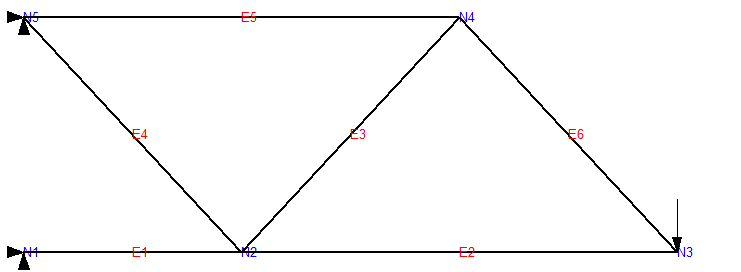
\includegraphics[width=.80\textwidth]{images/truss5_given}
    \caption{Optimal Vertical Truss}
    \label{fig:truss5_given}
\end{figure}

\begin{table}[p]
	\centering
	\caption{Optimal Vertical Truss - Method of Joints Analysis}
	\label{tbl:indeterm_5}
	\vspace{6pt}
	\begin{tabular}{ccc}
		\toprule
		Element & Force (N) & Element Deflection (m) \\
		\midrule
		1 &  -3 &  3.947e-7 \\
		2 &  -1 & 2.63e-7 \\
		3 &  -1.4142 &   2.60e-7 \\
		4 &  1.41421 &  2.63e-7 \\
		5 &  5 & 5.26e-7 \\
		6 &  1.41421 &  2.60e-7 \\ 
		\bottomrule
	\end{tabular}
\end{table}


\subsection{Horizontal Truss Analysis}
\label{sec:IDontCare}

Design one from section \ref{sec:3analysis} (figure \ref{fig:hz1}) was analyzed using the Method of Joints to validate the finite element analysis results.
The force and deflection for each member is shown in table \ref{tbl:horizontalAnalysis}; refer to figure \ref{fig:horizontalDiagram} for a diagram of the structure and labeled elements.
The overall deflection of 0.0409 mm under a load of 5 N compares well with the results obtained using finite element analysis.
The structure analyzed is somewhat different from that constructed and seen in figure \ref{fig:diagram}.
Many short members in the vicinity of the motor mount were neglected.
Additionally, the position of reaction forces were changed such that they occur at joints, not the actual position of the washers.
These simplifications were necessary to make the structure determinate and were required for many of the assumptions of the analysis, such as pin joints.
Refer to the appendix for calculation details.
%TODO HIGHPRI: Why valid
%Given the 

\begin{figure}[p]
    \centering
    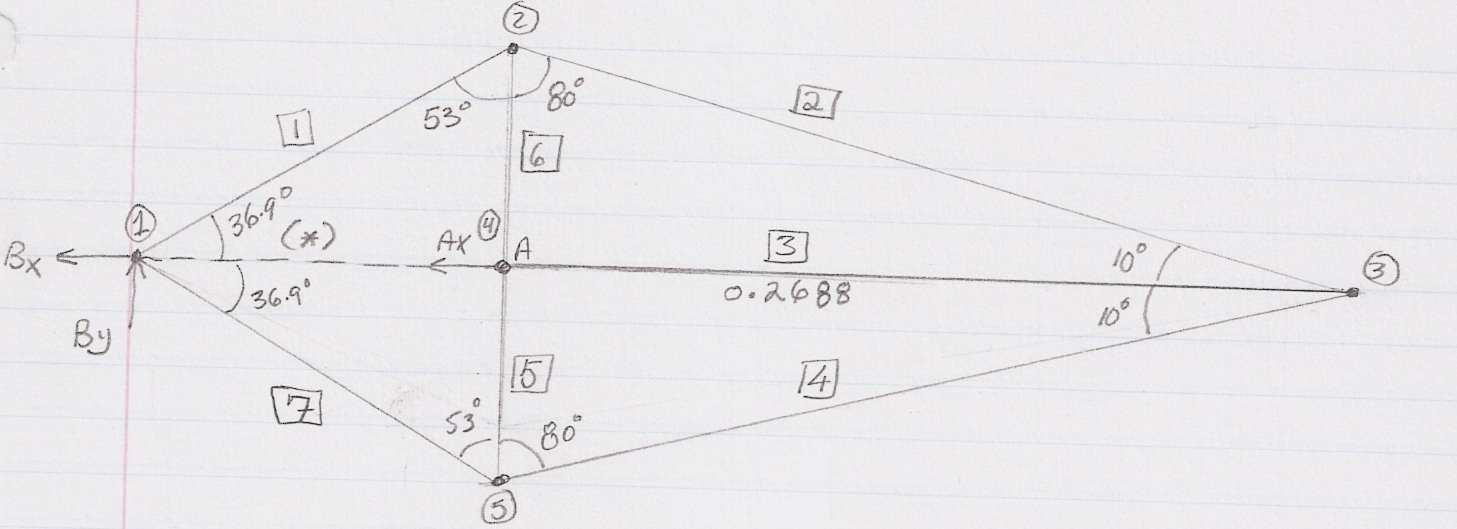
\includegraphics[width=.80\textwidth]{images/horizontalDiagram}
    \caption{Horizontal Truss Member Diagram} %TODO: change
    \label{fig:horizontalDiagram}
\end{figure}

\begin{table}[p]
	\centering
	\caption{Element Forces and Deflections (See figure \ref{fig:horizontalDiagram})}
	\label{tbl:horizontalAnalysis}
	\vspace{6pt}
	\begin{tabular}{rccc}
		\toprule
		Element & Force& Deflection  \\
		\midrule
		1 &  17.8sin(37)  &  1.11e-6 \\
		2 &  14.4 cos(80)  &  1.206e-5 \\
		3 &  0                    &  0 \\
		4 &  -14.4 cos(80)  &  -1.206e-5 \\
		5 &  13.2              &  8.16e-7 \\
		6 &  -13.2            &  -8.16e-7 \\
		7 & -17.8sin(37) & -1.11e-6 \\
		\bottomrule
	\end{tabular}
\end{table}